\chapter{Implementación} 
\label{f.implementacion}
\section{Capturas de pantalla} 
\label{f.implementacion.capturas}
A continuación se encuentran algunas capturas de pantalla de la aplicación en su estado final. 

\par
\begin{figure}[!h]
    \centering
    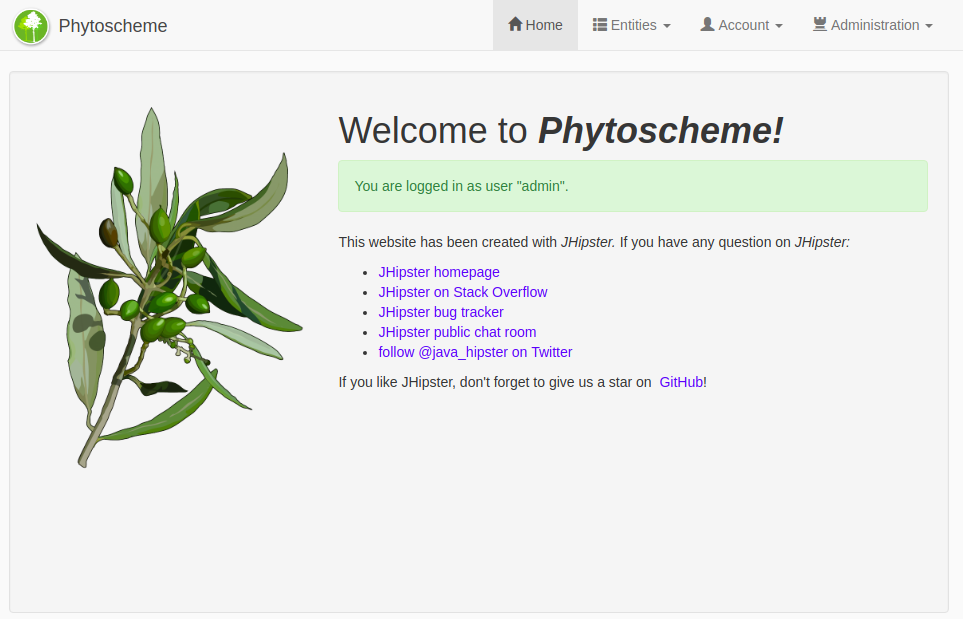
\includegraphics[width=\textwidth,height=\textheight,keepaspectratio]{Imagenes/Captura1}
    \caption{Captura de pantalla de la página de inicio de la aplicación \textit{Phytoscheme}.}
    \label{fig:capturaInicio}
\end{figure}

\par
\begin{figure}[!h]
    \centering
    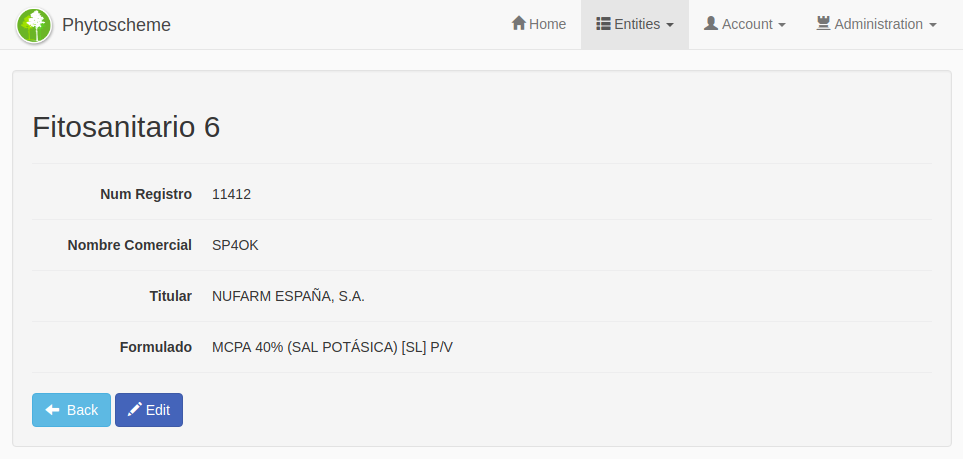
\includegraphics[width=\textwidth,height=\textheight,keepaspectratio]{Imagenes/Captura4}
    \caption{Captura de pantalla de la información de un producto fitosanitario.}
    \label{fig:capturaFitoDetalle}
\end{figure}


\par
\begin{figure}[!h]
    \centering
    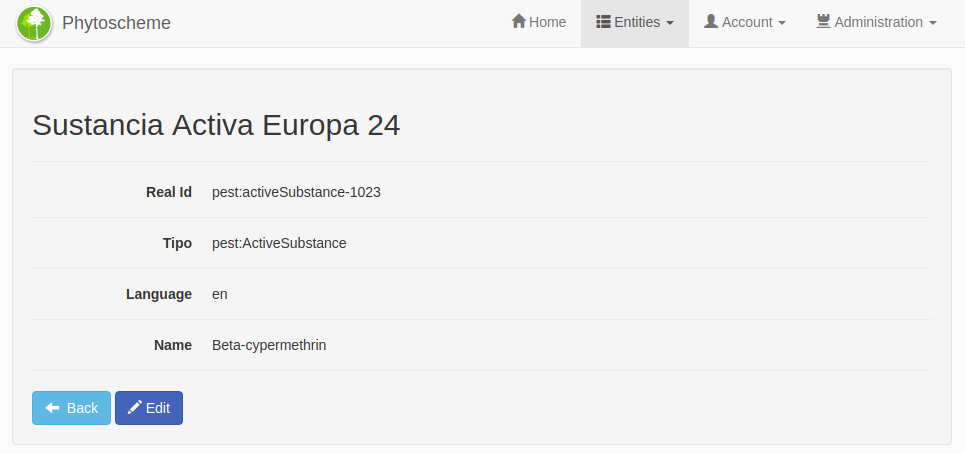
\includegraphics[width=\textwidth,height=\textheight,keepaspectratio]{Imagenes/Captura5}
    \caption{Captura de pantalla de la información de una sustancia activa.}
    \label{fig:capturaSustActDetalle}
\end{figure}